%%%%%%%%%%%%%%%%%%%%%%%%%%%%%%%%%%%%%%%%%%%%%%%%%
% Relatório Final - Projeto de Pesquisa
% Métodos de Otimização
% Baltz & Machado
% Capítulo 2
%%%%%%%%%%%%%%%%%%%%%%%%%%%%%%%%%%%%%%%%%%%%%%%%%

\chapter{\Large{Métodos Clássicos de Otimização}}\label{chp:2}


\section{{O Método de Newton}}

% TODO: Adicionar texto entre o início do cap e início da sessao
% Talvez falar sobre newton, sobre a criação do método, e tals
% Fazer a introdução

\subsection{Entendendo o Método}

\hspace{0.8cm}
O Método de Newton, foi desenvolvido com o objetivo de encontrar estimativas
para as raízes de uma função. De modo que, a execução do método é feita de
forma iterativa, repetindo sempre o mesmo processo, atualizando o mesmo valor.

Este método faz uso do recurso de derivação. Existindo uma relação muito
forte com o ângulo da reta tangente à curva, que é o gráfico da função que
foi derivada. Ademais, é importante ressaltar a necessidade de um ``palpite''
inicial, que represente o valor de \textit{x}, para o qual será buscado uma
estimativa da raiz. E com isso vamos entender como o método funciona.

O método em princípio consiste na utilização da reta tangente à um
ponto sobre à curva, para gerar valores cada vez mais próximos da raiz
daquela função. Analisamos a interseção da reta tangente com o eixo das
abscissas. Obtendo o ponto P1($x_p$, $y_p$). O novo valor de entrada na função
será construído com base nas coordenadas desse ponto.

A equação da reta que passa por um ponto de coordenada ($x_0$, $y_0$) é dada
por:

\begin{equation}
    (y - y_0) = m(x - x_0).
\end{equation}

E levando em conta que temos como objetivo encontrar $x$, que é um ponto
sobreposto no eixo x, podemos considerar $y=0$. Logo:

\begin{equation}
    -y_0=m(x-x_0).
\end{equation}

Com isso sabemos que $y_0$ é a imagem da função $f(x_0)$, e $m$ representa o
ângulo da reta tangente ao ponto ($x_0$, $y_0$). Como vimos no Capítulo 1,
 $m=f'(x_0)$. Desenvolvendo essa equação, temos:

\begin{equation}
    -f(x_0) = f'(x_0)(x-x_0),
\end{equation}

\begin{equation}
    -f(x_0) = f'(x_0)x - f'(x_0)x_0,
\end{equation}

\begin{equation}
    0 = f'(x_0)x - f'(x_0)x_0+f(x_0),
\end{equation}

\begin{equation}
    0 = x - x_0 + \frac{f(x_0)}{f'(x_0)},
\end{equation}

\begin{equation}
    x = x_0 - \frac {f(x_0)}{f'(x_0)}.
\end{equation}\\

Exemplificaremos no gráfico a seguir. Considerando a função $f(x)=-x^2+2x$, e
que o palpite inicial é $x_0=1.5$. $P1$ representa o ponto quando aplicamos
$x_0$ a $f(x)$. Podemos observar que como fruto da intersecção da reta tangente
em azul encontramos o valor $x_1$ que será usado na próxima iteração.

\begin{figure}[ht]
    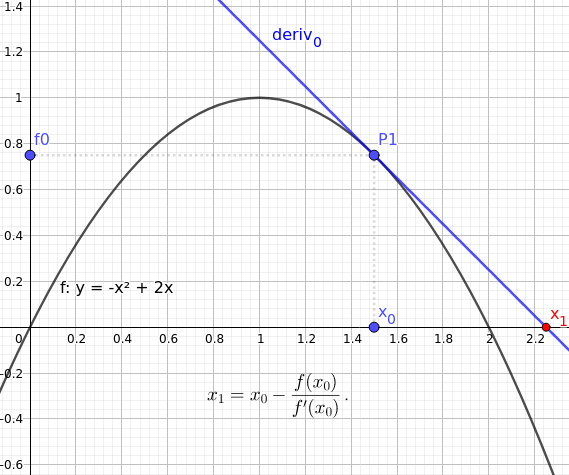
\includegraphics[width=0.55\textwidth]
      {src/MetodoNewton_grafico_1.png}
    \centering
    \caption{
      Primeira iteração do Método de Newton.
     }
    \label{MetodoNewton_grafico_1}
\end{figure}


Agora podemos entender melhor como a iteração funcionará. O valor
gerado, $x_1$, será aplicado no mesmo procedimento. E, a partir disso,
poderemos construir as seguintes equações:

\begin{equation}
    x_{1} = x_{0} - \frac {f(x_{0})}{f'(x_{0})},
\end{equation}

\begin{equation}
    x_{k+1} = x_{k} - \frac {f(x_{k})}{f'(x_{k})}.
    \label{newton_primeiraDeriv}
\end{equation}

% TODO: Provar o Teorema de Convergência do Método de Newton, escrever o
%teorema lá no final (do tópico ou do capítulo)

Desse modo, gera-se uma sequência $\{x_k\}$, que deve convergir para a
raiz da função (este é o cerne do Teorema de Convergência do Método de Newton).
Reconsiderando a função $f(x)$ do exemplo mostrado na Figura
\ref{MetodoNewton_grafico_1}, encontramos a pŕoxima iteração que apresentamos
na Figura \ref{MetodoNewton_grafico_2}:

\begin{figure}[h]
    \centering
    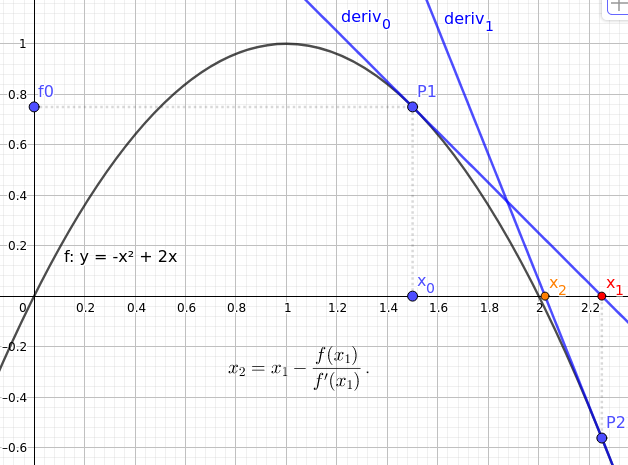
\includegraphics[width=0.55\textwidth]
      {src/MetodoNewton_grafico_2.png}
    \caption{
      Segunda iteração do Método de Newton.
    }
    \label{MetodoNewton_grafico_2}
\end{figure}

\newpage
Podemos notar que $x_2$ é um ponto mais próximo da raiz $f(x)$ do que $x_1$
ou $x_0$. O que evidencia a provável convergência da sequência $x_k$ para a
raiz.

É válido ressaltar que o denominador da equação
\ref{newton_primeiraDeriv} tem que ser diferente de 0 (ou seja, a reta tangante
num ponto $P$ não pode ser paralela ao eixo x). Caso contrário, teríamos
que a dada função não possui raiz na proximidade daquele ponto. Ademais, o
palpite, denotado por $x_0$, deve ser suficientemente próximo das raizes, para
garantir cerelidade da convergência.

Para aprimorar os resultados expostos, descrevemo-los como no seguinte teorema:

aloo
% TODO: Escrever aqui o teorema de Newton e a demonstração


\subsection{Encontrando Mínimos}

% TODO: Arruamar esse paragrafo

\hspace{0.8cm}
Agora podemos utilizar este método para encontrar mínimos de uma função.
O Método de Newton calcula raízes. É possível vincular isto, com o que
foi estudado no Capítulo 1. Obtemos os mínimos de uma função que como vimos
podem ser representados como raízes de sua derivada. Considerando $g(x)$ uma
função duas vezes diferenciável, e tendo como objetivo encontrar seus pontos
de mínimo, pode-se utilizar o Método de Newton para resolver tal problema o
que gera a seguinte sequência:

%TODO: Falar mais/melhor sobre a sequencia {x_k} (tendencia ao 0 da função)

\begin{equation}
    x_{k+1} = x_{k} - \frac {g'(x_{k})}{g''(x_{k})}.
    \label{convergencia_segundaDeriva}
\end{equation}

A convergência da sequência \ref{convergencia_segundaDeriva}, é um valor $x^*$
que satisfaz a equação:

\begin{equation}
    g'(x^*) = 0.
\end{equation}

O método é simples, entrega muitas vezes ótimos locais próximos ao ponto
inicial, mas tem seu destaque, que é ser, facilmente computável.

Problemas de maximização podem ser vistos sob o seguinte olhar:

\begin{equation}
    max(f(x)) = min(-1 * f(x)).
\end{equation}

O que faz com que o Método de Newton possa ser utilizado em ambos sentidos no
processo de otimizar.

O movimento de \(x_k\) dentro da sequência, é determinado pela relação das
quantidades e propriedades, que tanto a primeira quanto a segunda derivada
oferecem. As quantidades, determinam a velocidade do movimento, e os sinais,
indicam a direção do movimento. De certa forma, podemos interpretar o movimento
da sequência \(\{x_k\}\) como instantes do movimento de uma bola numa ladeira,
que no começo de sua descida é acelerada, e, conforme chega ao plano no fim da
ladeira, começa a reduzir sua velocidade, até supostamente chegar no ponto mais
baixo.


\section{{Outros Métodos}}

\hspace{0.8cm}
Com o advento do Método de Newton, acabou surgindo uma família de métodos
similares. E como foi visto, é possível a partir dele, encontrar tanto raízes
de funções, quanto máximos ou mínimos, tal característica é herdada pelos vários
métodos que deviram dele. Dentre eles temos; Métodos Quasi-Newton e Método do
Gradiente Descendente. Tais métodos podem ser vistos como uma complementação ao
Método de Newton, no entanto, esses fornecem uma grande flexibilidade em
como deseja-se utilizar os recursos de precisão e poder computacional.

Métodos Quasi-Newton se fazem necessários, quando nem sempre se tem acesso ou
recursos suficientes para se calcular a derivada de segunda ordem, ou até mesmo
a de primeira ordem. Já os métodos do Gradiente Descendente, como sugerido pelo
nome, utiliza-se majoritariamente, da derivada de primeira ordem em seu
processo.

% TODO: Está escrito por ordem de apresentação por paragrafo::::
% TODO: Citaritar nossos métodos [colocar que serão explicados melhor no cap tal])
% TODO: Falar sobre o Simplex aqui e outros métodos
% TODO: Informar que vamos falar especificamente dos 3 metodoss(newton,
% gradiente e simplex)
Os quais, descreveremos em alguma escala nas sessões seguintes.

\subsection{Métodos Quasi-Newton e Gradiente Descendente}

\hspace{0.8cm}
Aqui voltaremos a considerar uma função $f(x)$. E considerando que o Método
de Newton encontra o \(min(f(x))\) através de uma sequência \(\{x_k\}\):

\begin{equation}
    x_{k+1} = x_{k} - \frac {f'(x_{k})}{f''(x_{k})}.
\end{equation}

A qual, pode ser reescrita da seguinte forma:

\begin{equation}
    x_{k+1} = x_{k} -  \frac{1}{f''(x)} * f'(x_{k}).
\end{equation}

Sabemos que quem determina a direção da convergência é \(f'(x)\), portanto
não é completamente necessário o uso de \( \frac{1}{f''(x)} \), que
tem como principal papel controlar o tamanho do ``passo dado'' na iteração.
De modo que, a maioria dos Métodos Quasi-Newton fazem a substituição
da dada fração por aproximações boas o suficiente. E com isso, levando em
conta $\alpha$ como a representação dessa aproximação, temos:

\begin{equation}
    x_{k+1} = x_{k} -  \alpha * f'(x_{k}).
    \label{newton_lambda}
\end{equation}

Onde \(\alpha\) satisfaz:

\begin{equation}
    f(x_{k+1}) = f(x_{k} -  \alpha * f'(x_{k})) < f(x_{x}).
    \label{newton_restricao_alpha}
\end{equation}

A partir da equação \ref{newton_lambda}, podemos escolher um \(\alpha\), de
modo que, seja menos custoso encontrá-lo do que calcular a segunda derivada
da função objetivo, ou até, podemos nem calculá-lo, basta considerar
um \(\alpha\) fixo, e tão pequeno que, quando a restrição
\ref{newton_restricao_alpha} não for cumprida, já temos uma aproximação boa o
suficiente para o mínimo da função.

Podemos dizer que, esse modelo de resolução é útil e flexível o
suficiente. Tendo isso em mente, e seguindo para o problema de encontrar
o melhor \(\alpha\), já sabemos que sendo um valor pequeno o
suficiente, minimiza a função (mas, não da melhor forma). Já é sabido
que o \(\alpha\) tem como propósito, regular o tamanho do passo dado nas
iterações. Ele pode ser usado em conjunto com outros elementos, afim de
otimizar o processo de otimização.

Comumente usamos algum dos seguintes métodos para encontrar o tamanho do
passo:

    \begin{itemize}
            \item Um valor fixado para \(\alpha\);
            \item Um método que atualize \(\alpha\) de acordo com alguma
                situação;
            \item Um método que escolha um valor ótimo ou quase ótimo para
                \(\alpha\);
            \item Um elemento que forneça mais informações sobre a função,
                trabalhando em conjunto com algum \(\alpha\) definido nos
                métodos anteriores.
    \end{itemize}


Simplesmente considerando \(\alpha\) fixo e pequeno pode funcionar,
mas não seguramente para qualquer situação. Como por exemplo, uma função que
possui ``movimentos bruscos'', em um escala minúscula. Ou ainda, caso se tenha
considerado um ponto inicial muito distante de qualquer ótimo, resultando
em um funcionamento extremamente custoso do algoritmo.

Atualizar o valor de \(\alpha\), de acordo com a situação do processo iterativo
de otimização, pode ser uma boa opção, quando não se tem tanto poder
computacional. Comumente, pode ser encontrado implementações, que iniciam
com um \(\alpha\) não tão pequeno (isso ajuda a resolver o problema de
iniciar com um ponto longe da solução), mas ao passar das iterações,
reduz-se o seu valor por algum fator. Fator este, que pode ter alguma relação
com a magnitude da derivada, já que, ela pode nos dar uma dica do quão longe
o ótimo está do ponto atual, ou ainda, considerar o fator de redução havendo
uma relação com a iteração atual. Como por exemplo se considerarmos um
\(\alpha_0 \in \mathbb{R}^{+}\) e \(k \in \mathbb{N} \) poderemos considerar
a k-ésima iteração como:
% TODO: Colocar referencias aqui e em todo o resto
\begin{equation}
    \alpha_{k+1} = \frac{\alpha_{k}}{k},
\end{equation}
ou ainda:

\begin{equation}
    \alpha_{k+1} = \frac{\alpha_{0}}{2^k}.
\end{equation}

Vale a pena ressaltar os métodos mais famosos para tal tipo de atualização,
que também podem ser chamadas de clássicos por serem um ponto inicial, como por
exemplo, o método de Barzilai–Borwein, que pode ser considerado uma atualização
ingenua, porém efetiva e barata de realizar o cálculo. O \(\alpha\) é dado
pela seguinte expressão:

\begin{equation}
    \alpha_{k+1} = \frac{\langle \Delta x, \Delta g \rangle}
        {\langle \Delta g, \Delta g \rangle},
\end{equation}
onde \( \langle \cdot, \cdot \rangle \) significa o produto interno entre
vetores (no caso de funções que possuem uma variável apenas, podemos
considerar um vetor de apenas uma entrada), e:

\begin{equation}
    \begin{array}{ccc}
        \Delta x& = &x_k - x_{k-1},\\
        \Delta g& = &g_k - g_{k-1}.
    \end{array}
\end{equation}


Podemos considerar que \(g_k = f'(x_k) \) nos entrega a noção de direção de
descida, noção essa, que ainda pode ser melhorada, como veremos mais a frente.
Então, por agora, podemos ficar com a ideia de que \(g_k\) é a direção de
descida apenas, independente da forma com que foi obtida.

%TODO: Applied Optimization] Liqun Qi, Kok Lay Teo, Xiao Qi Yang - Optimization
%and control with applications (2005, Springer) - libgen.lc.pdf, pag 277 do pdf
Tem-se mais alguns métodos semelhantes, como o método Polak-Ribière 1997 e
outro gerado pelos estudos de Fletcher e Reeves 1964. \ref{AppliedOptimization}.

Quando começamos a observar outras formas de melhorar o valor de \(\alpha\),
acabamos por entrar em uma recursão, pois começa um estudo sobre como
otimizar um parâmetro específico de um otimizador. Os métodos mais famosos que
buscam valores ótimos, ou quase ótimos para \(\alpha\), são os métodos
classificados como \textit{line search}. Os quais, normalmente, trabalham
com condições específicas sobre a otimalidade de \(\alpha\), como as condições
de Wolfe. Tais métodos utilizam-se dos artifícios citados
anteriormente, já que, são uma peça básica na construção do otimizador,
ou ainda, podem utilizar métodos fora da família dos newtonianos.

Agora, antes de seguirmos para a analise de estatégias para obter um melhor
resultado, se faz necessária uma nova observação sobre a estrutura básica
dos métodos. Até o momento, viemos considerando apenas a derivada de primeira
ordem como sendo a direção certa a ser tomada. Vamos observar a seguinte
equação:

\begin{equation}
    x_{k+1} = x_{k} - \alpha * \frac{1}{f''(x_k)} * f'(x_k).
\end{equation}

Se tomarmos \(\alpha = 1\), temos o método em sua forma natural. Mas
podemos procurar um valor para \(\alpha\) que melhore ainda mais a iteração.
E, complementando, sabemos sobre as acusações que a derivada de segunda ordem
faz sobre a otimalidade, com isso podemos dizer que a direção de otimização
em verdade é dada por:

\begin{equation}
    g_k = \beta(x_k) * f'(x_k).
\end{equation}

Então podemos reescrever a sequência de iteração na seguinte forma:

\begin{equation}
    x_{k+1} = x_{k} - \alpha * g_{k}.
\end{equation}


Daí, temos normalmente três opções no que diz respeito ao \(\beta(x_k)\),
que são:

\begin{enumerate}

    \item Considerar \(\beta(x_k) = \frac{1}{f''(x_k)}\). O que
        nos dá o Método de Newton novamente, e o \(\alpha\) não passaria de
        um mero ajuste;

    \item Considerar
        \(\beta(x_k) \approx \frac{1}{f''(x_k)}\). O que abre um leque de
        possibilidades no que diz respeito ao cálculo dessa aproximação
        e tornando-o assim num método Quasi-Newton. Sendo esse formato um dos
        mais populares. São aplicados nos métodos de otimização
        padrão em bibliotecas cientificas, como \textit{scipy} em Python,
        e \textit{GSL} em C. Tendo como um dos mais famosos o método BFGS
        (Broyden-Fletcher-Goldfarb-Shanno).

    \item Considerar \(\beta(x_k) \) neutro. O que possibilita considerar
        \(g_k\) = \(f'(x_k)\). Dando-nos o Método do Gradiente Descendente
        que, como dito anteriormente, normalmente é resolvido usando a
        estratégia de \textit{line search}.

\end{enumerate}

\subsection{Simplex}

\hspace{0.8cm}
O Método Simplex pode ser classificado como clássico, por ser um
dos métodos mais famosos. Formulado por George B. Dantzig, fruto de uma
sugestão de T. S. Motzkin, que contribuiu para diversas áreas da
matemática.

Os problemas que o Método Simplex resolve fazem parte de um conjunto de
problemas de Otimização Linear (ou Programação Linear). Os quais se restringem
apenas funções lineares. Além disso, tais problemas genericamente acompanham
restrições sobre as entradas da função a ser otimizada.

Um problema de otimização linear pode ser transcrito da seguinte forma.
Considerando a função objetivo:

\begin{equation}
        Z = c_1x_1 + c_2x_2 + … + c_nx_n,
\end{equation}
e tendo restrições também lineares para a função objetivo, como por exemplo:

\begin{equation}
    \begin{array}{ccc}
        &   a_{11}x_1 + a_{12}x_2 + … + a_{1n}x_n \leq b_1,\\
        &   a_{21}x_1 + a_{22}x_2 + … + a_{2n}x_n \leq b_2,\\
        &   ...\\
        &   a_{m1}x_1 + a_{m2}x_2 + … + a_{mn}x_n \leq b_m.\\\\
        &   x_1 \geq 0, x_2 \geq 0, …, x_n \geq 0.
    \end{array}
\end{equation}

O tipo de problema que o Simplex resolve, se desenvolve como a seguir:

\begin{equation}
        max \{c^tx | Ax \leq b, x \geq 0\}\\
\end{equation}


A forma de operação desse método é semelhante ao que uma pessoa comumente
faria ao se deparar com o problema de forma gráfica. O problema, que é
completamente linear, gera retas que acabam por formar regiões de
possíveis soluções, e dessas regiões, o que queremos é saber qual a melhor
solução. Para isso, bastaria procurar dentro de tal região, onde o valor da
função objetivo Z é o maior possível. Uma vez que a região tenha sido
construída pelas retas, teremos a característica de ser convexa, como um
polígono convexo no plano ou um poliedro convexo no espaço. O que acaba
facilitando a busca pelo máximo, dentro dessa região, uma vez que basta olhar
os vértices de tal região. Esses fatos podem ser provados e tais demonstrações
podem ser encontradas em [??].
% TODO: Colocar aqui uma boa referência (ou mais de uma)

Repara-se que o Método Simplex não se utiliza de artifícios e ferramentas do
Cálculo, como nos métodos anteriormente apresentados, mas sim, de formas
diferentes de analisar o problema, que por certos aspectos é simples. O método
completo é constituído por operações em uma matriz específica, denominada
Tableau, que representa o problema, o qual não é necessário ser apresentado
aqui, por se distanciar da ``família'' de métodos de otimização que é nos
interessa apresentar.


\section{{Programando os Métodos}}

% TODO: Colocar um texto aqui introduzindo o tópico
% Podemos falar de linguagens, e tals;;; Podemos falar também sobre as
% dificuldades de representar um método de otimização. Falar também das
% vantagens de utilizar tal linguagem

\hspace{0.8cm}
\subsection{Método de Newton}

\hspace{0.8cm}
A forma mais simples e mais útil de implementar o Método de Newton é na
busca das raízes da derivada da função objetivo. Que uma vez implementada
precisamos por como entrada a primeira e a segunda derivada da função que
desejamos minimizar, já que o método não precisa saber qual a função de fato.
A seguir temos a implementação na linguagem de programação \textit{Rust}:
\vspace{0.2cm}
\begin{lstlisting}
pub fn newton1x1<F>(funcao_derivada: &F, x: f64) -> (usize, f64)
where
    F: Fn(f64) -> f64,
{
    let mut entrada_atual = x;
    let maximo_iteracoes = 100;

    for iteracao_atual in 1..=maximo_iteracoes {
        let diferenca: f64 =
            funcao_derivada(entrada_atual.clone())
            /
            derive1x1(&funcao_derivada, &entrada_atual);

        println!("diferenca: {}", diferenca);
        entrada_atual -= diferenca;

        if diferenca.abs() < 0.0000001 {
            return (iteracao_atual, entrada_atual);
        }
    }

    return (maximo_iteracoes, entrada_atual);
}
\end{lstlisting}


Esta implementação define um procedimento que encontra alguma raiz de uma função
$f$. Que tem os seguintes parâmetros:

    \begin{itemize}
        \item A função $f$ tem como domínio um intervalo
            \(\mathbb{I} \subseteq \mathbb{R}\) e imagem um valor Real;

        \item E uma entrada $x$ sendo como o ``palpite'' inicial do ótimo.
    \end{itemize}


Além disso, temos o procedimento \textit{derive1x1}, que recebe como parâmetro
uma função e um valor $x$, tendo como retorno a derivada da função entregue
no ponto especificado. Restringindo-se à funções do tipo
\(f : \mathbb{I} \subseteq \mathbb{R} \rightarrow \mathbb{R}\).


\subsection{Método do Gradiente Descendente}

\hspace{0.8cm}
A implementação desse método exige apenas que seja definido o cálculo
da derivada da função objetivo, o valor de $\alpha$, um palpite inicial para
o valor de x e a quantidade de iterações desejada. Também, pode ser
indicado um valor que se refere à diferença dos dois últimos valores
da sequência \{$x_k$\}, podendo assim efetuar a parada da execução do
método. A seguir, temos a implementação na linguagem de programação
\textit{C++}:

\vspace{0.2cm}
\begin{lstlisting}[language=C++]

// Sendo f(x) = x^4 - 3*x^3 + 2
#include <bits/stdc++.h>
#define decimal long double
using namespace std;
// Calcula a derivada da funcao
decimal df(decimal x) {
	return 4 * pow(x, 3) - 9 * pow(x, 2);
}
int main() {
	// Palpite inicial
	decimal x_proximo = 5.5;
	// Variavel para iterar
	decimal x_atual;
	// Quantidade maxima de iteracoes
	int iteracoes = 100000;
	decimal alpha = 0.00001;
	// Precisao para condicao de parada
	decimal precisao = 0.000000001;
	// Comeca as iteracoes
	while(iteracoes > 0) {
		x_atual = x_proximo;
		x_proximo = x_atual - (alpha * df(x_atual));
		decimal precisao_atual = x_atual - x_proximo;
		// Se atingir a precisao desejada
		if(abs(precisao_atual) < precisao)
			break; // Para as iteracoes
		// Conclui uma iteracao
		iteracoes -= 1;
	}
	cout << ``x que minimiza f(x) = '' << x_proximo << endl;
	// Saida do algoritmo:
	// --> x que minimiza f(x) = 2.25
	return 0;
}


\end{lstlisting}



\textcolor[rgb]{1,0,0}{\section{{O Método de Newton para Várias Variáveis}}}
